\chapter{Realisation et implementation de l'application mobile}
\label{sec:Realisation de l'application mobile}

\section{Renewal}

\subsection{Les systèmes de recommandation}
Les systèmes de recommandation sont une forme spécifique de filtrage de l'information (SI) visant à présenter les éléments d'informations (films, musiques, livres, news, images, pages Web, etc) qui sont susceptibles d'intéresser l'utilisateur. Généralement, un système de recommandation permet de comparer le profil d'un utilisateur à certaines caractéristiques de référence et cherche à prédire l'« avis » que donnerait un utilisateur. Ces caractéristiques peuvent provenir de:

\begin{itemize}
    \item l'objet lui-même, on parle « d'approche basée sur le contenu » ou content-based approach. 
     \item L'utilisateur. 
    \item  l'environnement social, on parle d'approche de filtrage collaboratif ou collaborative filtering.

\end{itemize}

\subsection{Concurrence et la solution renewal}
Les recherches dans le domaine des systèmes de recommandation s’appuient la plupart du temps sur des évaluations “offline” qui ne permettent pas d’établir des métriques en phase avec une réelle satisfaction utilisateur. Dans le sous-domaine de la recommandation d’articles d’actualité, il existe à ce jour très peu de système permettant aux différentes équipes de recherche de tester leurs algorithmes en temps réel, i.e. sur des utilisateurs interagissant directement avec le système de recommandation.


La NewsREEL Live Task \cite{clef-newsreel} est, à notre connaissance, le seul système permettant de confronter différentes équipes sur des données en temps réel. Cependant, ce système est contraint sur plusieurs plans :

\begin{itemize}
    \item les données et le tracking des utilisateurs sont limités et ne permettent pas des recommandations à long terme. 
    
    \item  il n’existe pas d’interface dédiée à la recommandation et proposant des articles provenant de différentes sources.

\end{itemize}

Le projet Renewal se concrétise par le développement d'une application qui devra permettre de contourner les contraintes citées pour NewsReel Live Task et de permettre l'évaluation de nos algorithmes de recommandation sur des utilisateurs en contexte et en temps réel. Par la suite, nous proposons de développer un système qui tentera de contourner ces obstacles, ce qui aménera à la confrontation de différentes équipes de recherche. L'ensemble de ces contraintes énoncées doivent être prise en compte dès le début du développement de l'application mobile.


\subsection{Le concept Renewal}

Le concept central est construit autour de 2 types de recommandations au sein d'une application mobile dédiée. Ce contexte permet une analyse riche et fine du comportement avec un large panel d’indice conceptuel comme la géolocalisation ou le niveau de batterie sur le long terme. La tâche principale de Renewal est de recommandées des nouvelles diverses recommandé spécifiquement pour un utilisateur donné. La liste d’article générée pour l’utilisateur est le fruit de deux systèmes de recommandation que nous appellerons A et B. Lorsque l’utilisateur fait défiler les articles ou choisi un article, le moindre mouvement dans sa navigation est finement analysé via le temps, la vitesse de défilement, le temps de lecture du titre et bien plus. L’analyse fine du comportement permet de connaitre si l’algorithme A est plus pertinent que l’algorithme B ou inversement et de remplacer l’algorithme le moins pertinent par un algorithme C. Cette compétition permettra de connaitre in fine le meilleur algorithme de recommandation dans le sous domaine de la recommandation d’article. Une tache secondaire mais extrêmement importante est la recommandation d’article complémentaire non redondant avec la liste d’article recommandée via la recommandation diverse et surtout de fournir des informations supplémentaires sur un article donné. La navigation d’articles complémentaires est imaginée comme un parcours d’article en article sous forme arborescente. 

\begin{figure}[htp]
  \centering
  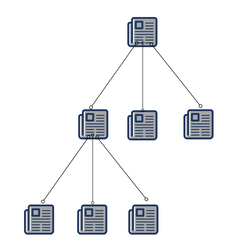
\includegraphics[width=7cm]{images/arbo}
  \caption{Methode arborescente}
  \label{fig:arbo}
\end{figure}


Renewal se veut être une plateforme modulaire où diverse équipe de recherche pourront proposer leur algorithme de recommandation d’article selon un contexte extrêmement riche et une base importante d’utilisateur. Cette expérience permettra aux équipes de recherches d’obtenir des statiques extrêmement complètes sur le résultat produit par leur algorithme à grande échelle.  


\section{Accès et analyse du comportement de l'utilisateur}

\subsection{User Cold Start}

En l’absence totale d’information sur l’utilisateur, la seule solution adoptée est d’utiliser des données externes, typiquement en s’aidant des informations sur les réseaux sociaux, c’est la direction que nous avons choisi pour l’application en accord avec la thèse préparée par Julien HAY. D’autres techniques s’appuient sur des méthodes spécifiques lorsque peu de données sont présentes, une review de ces méthodes est détaillée dans Dealing with the new user cold-start problem in recommender systems: A comparative review de Le Hoang So

L’idée est d’exploiter les posts et partages dans la recommandation pour résoudre la problématique du user cold start. Dans nos expérimentations, nous allons modéliser chaque type de contenu et chaque type d’interaction (partage, retweet, tweet, citation...) selon différentes pondérations et créer un vecteur représentatif des utilisateurs en utilisant des techniques de text embedding conditionnées par les triplets user-interaction-content. Nous appuierons nos travaux sur l’article Analyzing user modeling on Twitter for personalized news recommendations (2011) \cite{Analyzing} qui prend en compte les posts utilisateurs dans de la news recommendation et Improving User Topic Interest Profiles by Behavior Factorization (2015) \cite{User} qui séparent le contenu par type d’interaction.



\subsection{Gestion du compte utilisateur}

Au sein de notre application, nous avons choisi de laisser le choix à l'utilisateur d'utiliser soit une simple inscription par mail soit via un réseaux social. L'inscription via un simple mail rend plus complexe l'analyse des recommandations puisque nous avons aucune information complémentaire permettant de recommander des articles pertinents pour ce dernier. Au contraire, la connexion via Google, Facebook et Twitter permet selon les droits accordés à notre application Renewal de disposer de plus d'information concernant notre futur utilisateur. Ce type de connexion est de plus en plus plébiscité par les utilisateurs dont l'inscription à un contenu s'effectue en quelque seconde sans avoir besoin de rentrer son adresse mail et son mot de passe dans la plupart des cas où l'utilisateur est soit déjà connecté sur ce réseau ou dispose de l'application sur son smartphone.

\subsection{Evaluation du comportement et de la pertinance au sein de la recommandation}

Pour connaitre si un article est pertinent pour un utilisateur il faut étudier finement le comportement de l'utilisateur au sein de l'application. Dans un premier temps sur la liste d'article recommandé à l'utilisateur, il faut connaitre le temps passé sur la liste et les articles visibles pour l'utilisateur et à combien de pourcent. Si l’utilisateur passe un moment à regarder l’image et le titre de l’article ou au contraire il sélectionne très rapidement un article.

\begin{figure}[htp]
  \centering
  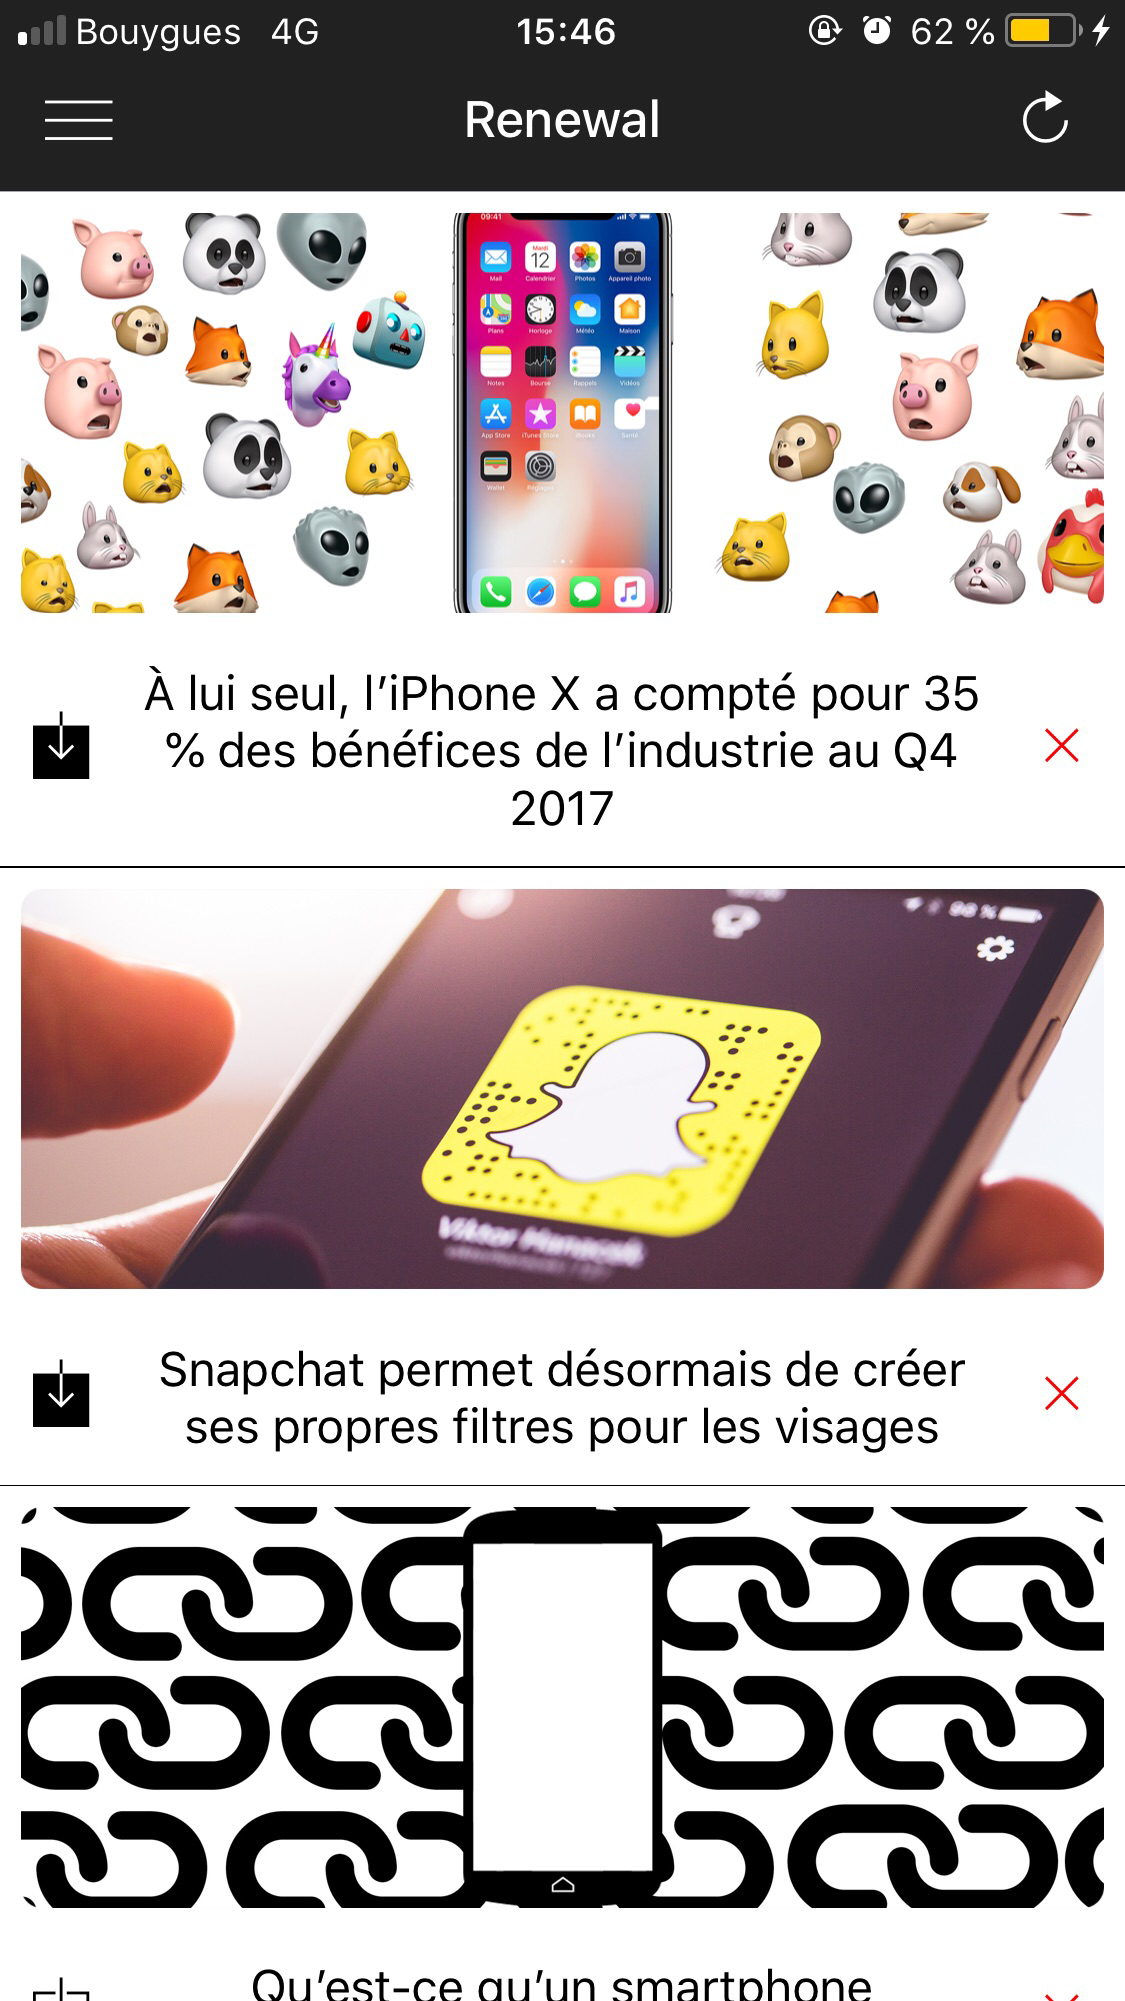
\includegraphics[height=10cm]{images/divers}
  \caption{Exemple de recommandation diverse.}
  \label{fig:screen-settings}
\end{figure}


Pour analyser le plus finement possible le comportement de l’utilisateur, il faut obtenir le maximum d’informations sur sa navigation et les conditions selon lequel il utilise l’application.  La récolte d’information peut s’effectuer via les différents capteurs disponibles sur le smartphone comme l’accéléromètre ou la localisation de l’individu nous permettant de proposer des actualités locales à l’utilisateur et de déterminer ses habitudes. La navigation au sein de la liste d’articles recommandés, notamment les articles visibles par l’utilisateur et à combien de pourcentage sont-ils visibles permet de savoir si la vignette de l’article, le titre de l’article ou les deux ont le plus d’importance pour l’utilisateur.  La détermination du temps passée sur la liste à son importance pour la détermination des articles recommandés.  
La récolte du plus d’information possible par utilisateur est extrêmement important pour les équipes de recherche et les capteurs permettent de savoir si l'utilisateur marche ou est simplement en mouvement. Les personnes en mouvement sont potentiellement susceptible de cliquer sur une vignette aguicheuse d’un article plutôt qu’un titre ou inversement cela sera déterminé par les équipes de recherche et leurs algorithmes de recommandation. La lecture d’un article sera aussi très finement analysée permettant de vérifier la pertinence de l’article via le temps passé à lire l’article ou si l’utilisateur à partagé l’article à un ami. En effet, si l’utilisateur reste 10 secondes sur l’article ce dernier n’est surement pas pertinent pour l’utilisateur.



\subsection{Loi RGPD}

Le Règlement général sur la protection des données (RGPD ou GDPR, pour General data protection régulation en anglais) est le nouveau cadre européen concernant le traitement et la circulation des données à caractère personnel, ces informations sur lesquelles les entreprises s’appuient pour proposer des services et des produits. Avant le RGPD existait une directive sur la protection des données personnelles qui date de 1995. Ce texte est abrogé par le RGPD. Le déploiement du RGPD dans l’espace européen se fait en deux temps : il y a d’abord eu, le 14 avril 2016, l’adoption définitive du texte par le Parlement. Cependant, son application ne s’est pas déroulée au même moment : il a été décidé de la décaler de deux ans, au 25 mai 2018 soit 2 mois après le début de mon stage. 


Du point de vue de l’internaute, le RGPD met en place ou conforte un certain nombre de protections. Il faut par exemple que les entreprises récoltent au préalable un consentement écrit, clair et explicite de l’internaute avant tout traitement de données personnelles, ou qu’ils s’assurent que les enfants en-dessous d’un certain âge aient bien reçu l’aval de leurs parents avant de s’inscrire sur un réseau social.

Le RGPD inclut aussi une reconnaissance d’un droit à l’oubli pour obtenir le retrait ou l’effacement de données personnelles en cas d’atteinte à la vie privée et le droit d’être informé en cas de piratage des données. Les internautes pourront aussi être défendus par les associations dans le cadre d’une action de groupe en vue de faire cesser la partie illicite d’un traitement de données.

Dans le cadre du développement de mon application mobile, j'ai exploité fortement les données issues des réseaux mais aussi l’analyse fine du comportement de l’utilisateur. Dans la loi RGPD, Facebook a durci l’accès aux données pour protéger ses utilisateurs. La rédaction d’un long dossier est nécessaire pour avoir accès à des données avancées (autre que le nom, prénom, email, date d’anniversaire) durant lequel il faut expliquer pour chaque donnée avancée l’utilisation faite par notre entreprise/application.  La rédaction de ce dossier permet à Facebook de s’assurer que notre application n’exploite pas les données de chaque utilisateur de façon abusive. Depuis l’entrée en vigueur de la loi RGPD, il est obligatoire de pouvoir laisser à chaque utilisateur l’accès ou non à chaque élément permettant le tracking d’un utilisateur et l’exploitation de ses données. Une autre notion obligatoire depuis la loi est de permettre à chaque utilisateur de récupérer l’ensemble des données rassemblées sur lui facilement.


\subsection{L'accès aux données sensibles et inconvéniants }

Pour avoir un système de recommandation pertinent, il est nécessaire d'avoir accès à certaine information dite sensible de l’utilisateur. Ces informations permettront aux algorithmes d'avoir un contexte pour chaque utilisateur permettant de déterminer si un article correspond plus ou moins à un utilisateur donné. Les données dites sensibles nous serons accessibles seulement via la connexion des différents réseaux sociaux faite par l'utilisateur. L'obtention des données autres que l’adresse et le nom d'utilisateur n'est pas obtenue via une connexion basique à l'aide d'un bouton sur notre application Renewal. 


Cet accès aux données sensibles est extrêmement complexe à obtenir et demande l'approbation du réseau pour chaque donnée de façon individuel. Certaine donnée extrêmement personnelle de l'utilisateur comme les posts du son mur Facebook demande l'élaborateur d'un dossier complet permettant de justifier l'accès aux données mais aussi le contexte global de l'application et la réelle utilité des données. Pour expliquer plus précisément ma démarche, je vais prendre pour exemple Facebook mais l'obtention des données sur les autres réseaux est sensiblement la même.


En première étape, il faut inscrire l’application sur la plateforme développeur du réseau social en renseignant les coordonnées du délégué à la protection des données (obligatoire depuis la loi RGPD) et des renseignements concernant l’application elle-même comme le domaine de l’application, son but, etc.  L’ensemble de ces renseignements fourni permettront d'obtenir un identifiant unique de l’application qui couplé à une clé secrète accordera par la suite une connexion à l'API. Pour pouvoir faire une connexion basique entre notre application et Facebook, il faut spécifier à partir de quelle plateforme l'utilisateur va se connecter. Dans notre cas, il s'agit d'Android et iOS, une clé secrète unique sera générée pour chaque plateforme et permettant de créer manuellement un bouton connexion avec Facebook ou si la connexion aboutie permettra de récupérer des informations basiques comme l'email, le nom d'usage et le prénom. Dans le contexte énoncé pour notre application, ce type de connexion est moyennement intéressante et ne permet pas de contrer le problème du User Cold Start.


La seconde étape est essentielle pour la viabilité de notre application et ainsi contourner le problème du User Cold Start. Cette étape consiste à obtenir l'accès via l'API Facebook d'obtention des données plus personnelles sur l'utilisateur permettant d'avoir des systèmes de recommandation pertinent et une expérience satisfaisante pour un utilisateur lambda. En fonction du type de données demandé, l'accès est plus ou moins facile à obtenir. Concrètement, connaitre la date de naissance ou le sexe de l'utilisateur est une donnée relativement simple à obtenir. Contrairement aux posts de l'utilisateur, le contenue "liker" par ce dernier ou les récents partages qui sont des données accessibles seulement pour une minorité d'entreprise cela est d'autant plus vrai depuis l'application de la loi RGPD. J'ai commencé par demandé l'accès aux données les moins contraignantes en termes d'accès par Facebook, la démarche est plutôt simpliste mais demande un long moment d'attention. Dans un premier temps, il faut spécifier dans quel cadre nous avons besoin de cette information, dans quel but et préciser avec exactitude à quel moment l’appel à ce type de donnée intervient et quel sont les changements pour l'utilisateur. Facebook peu alors procéder à la vérification du dossier et tester l’exécution des faits énoncés manuellement par un opérateur habilité. Il faut aussi fournir les exécutables de l'application ici le  .apk ou .ipa de l’application ainsi qu’une courte vidéo explicative permettant d'aider Facebook à reproduire avec exactitude le moment où l’appel aux données est nécessaire. La validation par Facebook étant au cas par cas non automatisée. La démarche peut prendre plusieurs semaines avant d’obtenir l’approbation ou le refus de Facebook auquel cas il faudra recommencer entièrement la seconde étape.


\subsection{Gestion des paramètres de l'application}

\begin{figure}[htp]
  \centering
  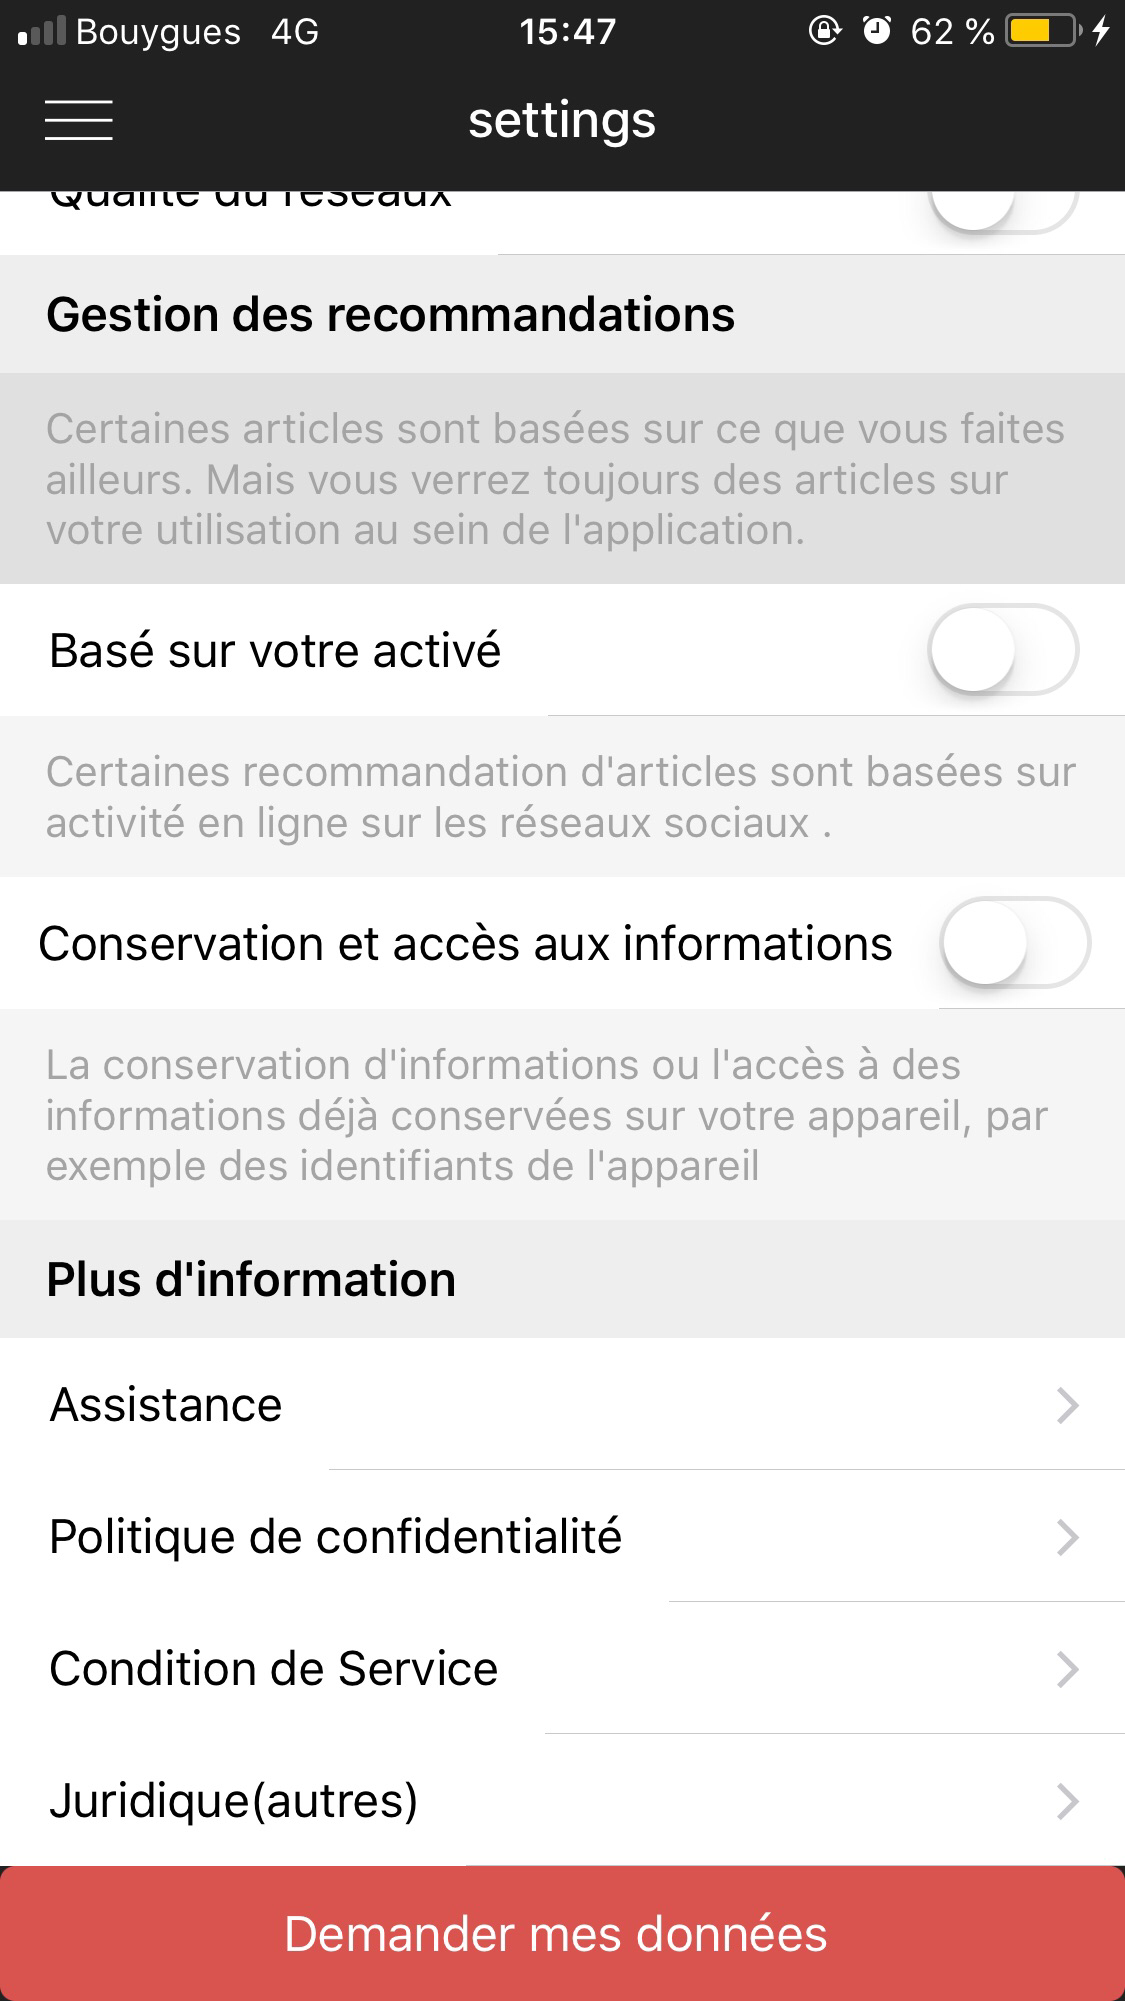
\includegraphics[height=10cm]{images/s2}
  \caption{Page des paramètres.}
  \label{fig:screen-settings}
\end{figure}

Depuis l'application de la loi RGPD, il est nécessaire d'offrir à l'utilisateur un droit de regard sur la gestion fine de ses données et d'expliquer dans quel but nous récoltons une information. Nous avons divisé la page de paramètres en trois sections :

\begin{itemize}
    \item La gestion des différents capteurs, permettant entre autres de connaitre la position de l’utilisateur et donc pour apporter plus d'informations contextuelles aux algorithmes de recommandation. 
     \item La gestion des recommandations, dans cette section permet de modifier l'accès aux données sur ses différents réseaux, ainsi que la conservation des données et le ciblage. 
    \item La section assistance et condition de service permettant à l'utilisateur d'obtenir plus d'informations sur l'application, son contexte et aussi de rentrer directement en contact avec l'équipe en charge du projet.

\end{itemize}




En bas de la page paramètres est disposé un bouton "Demander mes données" lui-aussi essentiel depuis la loi RGPD qui permet évidement l'envoi de l'ensemble des données récolté et stocké sur l'utilisateur depuis son inscription sur l'application Renewal. 

\section{Lecture d'un article}

\subsection{Analyse du comportement au sein d'un article}

Lorsqu'un utilisateur sélectionne un article, celui-ci est lancé dans une WebView. Nous avons fait le choix d'une WebView plutôt que l'extraction du contenue d'un article pour que l'utilisateur ne perde pas d'informations lors de la lecture d'un article puisque c'est le site dont l’article est issu donc l'information n'est pas détériorée ou coupée. L'utilisateur dispose donc un accès complet à l'article souhaité.

\begin{figure}[htp]
  \centering
  
\includegraphics[height=10cm]{images/webview}
  \caption{Exemple de WebView avec la languette.}
  \label{fig:screen-wv}
\end{figure}

La page de lecture est donc composée de deux éléments principaux mais aussi d'un composant crée par nos soins qui est "languette". La mise en place d'une WebView est aisée mais la communication entre notre application et la WebView fut compliquée à mettre en place. Notre WebView permet l'injection de JavaScript lors de l'exécution de la page. Le but est d'extraire un maximum d'information sur le comportement lors de la lecture d'un article comme le temps de lecture ou si l'utilisateur à parcouru l'ensemble de l'article. Pour les équipes de recherche, ces informations précieuses permettent de connaitre la pertinence de l'article vis à vis de cet utilisateur. Pour envoyer l'ensemble des informations regroupées dans la WebView à notre application j'utilise la fonction postMessage. Malheureusement toutes les fonctions relatives à l'envoi de message ne fonctionnent absolument pas et fait d'ailleurs l'objet de nombreuses issues sur le GitHub de React-Native. Face à ce problème deux solutions sont possibles la WebView va envoyer les paquets de données récoltées elle-même à un serveur, soit trouver une solution pour laisser l'application comme unique agrégateur de paquet. La première solution pose énormément de contrainte coté serveur comme faire concorder les flux en provenance de l'application et de la webView mais aussi donner à la WebView les moyens de se connecter au serveur. J'ai donc décidé de trouver une solution et contourner ce problème. A l'aide de la communauté GitHub, j'ai réussi à mettre en place un bridge dans l'envoi de message au sein de l'injection JS permettant l'envoi de données sous le format JSON. Une adaptation du code permettant la réception des messages a été nécessaire pour adapter la réception au format JSON. Cette étape à retardé la finalisation d'une semaine, le temps nécessaire à l'élaboration d'une solution viable. Aujourd'hui, cette solution est parfaitement fonctionnelle mais a nécessité l'ajout d'un tag afin de différencier les messages en provenance de notre analyse du comportement et ceux de certains sites.



Concernant la "languette", il s'agit d'un élément essentiel de notre application puisque la recommandation d'article complémentaire est faite à l'intérieur de cette languette. Le design final de la languette est le fruit d'une certaine réflexion. Il faut rendre cet élément non-intrusif lors de la lecture d'un article tout en insistant l'utilisateur à la découvrir. Nous avons choisi de minimiser au maximum l'espace pris par la languette à condition que celle-ci soit toujours swipable facilement. Une icone de flèche perpétuellement en mouvement indique à l'utilisateur la présence continuelle de la languette. 

Au sein de la languette, des éléments permettent de noter manuellement la pertinence de l'article et agiront de pair avec l'analyse faite automatiquement. Un bouton partage est disponible avec un certain nombre d'élément prérempli lors de l'envoi d'un article par mail ou par les réseaux sociaux. Ces éléments permettent de mettre en avant notre application lors des partages et donc l'augmentation de notre base d'utilisateur. Mais l'élément le plus important pour les équipes de recherche travaillant dans les systèmes de recommandation c'est la mise à disposition d'une liste d'articles complémentaires.


\subsection{La recommandation d'articles complementaires}

\begin{figure}[htp]
  \centering
  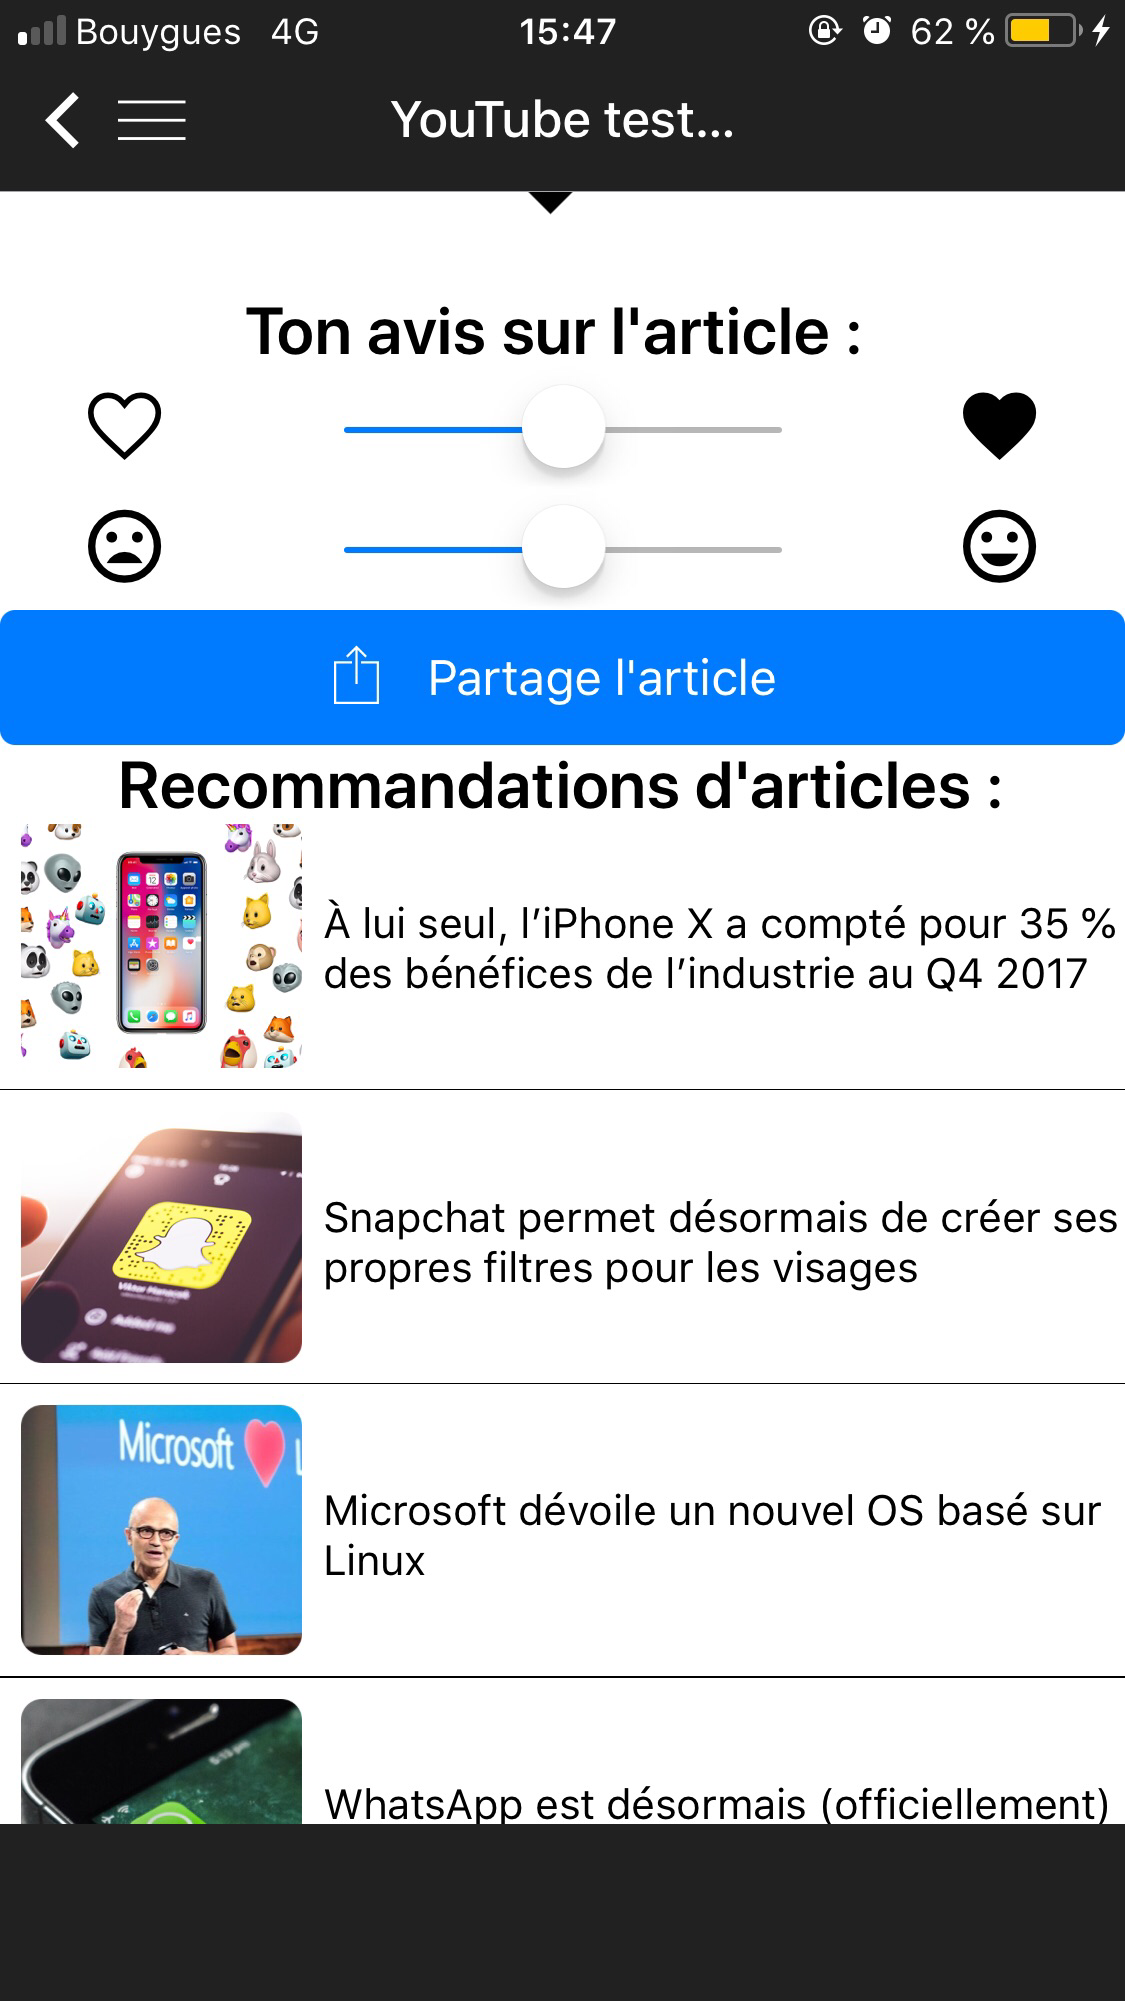
\includegraphics[height=10cm]{images/comp}
  \caption{Exemple de  recommandation de complementaire.}
  \label{fig:screen-comple}
\end{figure}


La tâche consiste à recommander des éléments d'actualités complémentaires à l'article actuel. Cette tâche est assez complexe puisque les articles proposés dans cette liste doivent apporter des informations complémentaires sans être redondant avec l'article actuel. De plus cette recommandation n'est pas considérée comme un élément secondaire de l'application mais un élément essentiel. D'un point de vue technique, la recommandation d'article complémentaire est imaginée comme une structure d'arborescence dans lequel l'utilisateur navigue d'articles en articles complémentaires et revient à la recommandation diverse une fois qu'il est suffisamment informé sur un sujet. Cette recommandation d'articles est un exercice complémentaire à la recommandation d'articles divers sur lequel les équipes de recherche seront mis aussi en compétition sur la pertinence et l'efficacité de leur algorithme.


%%% Local Variables: 
%%% mode: latex
%%% TeX-master: "lri-report"
%%% End: 